\documentclass[a4paper,12pt,polish]{book} % nie: report!
\usepackage{url}
% \usepackage{hyperref}



% \usepackage[polish]{babel}
% \usepackage[polish]{babel}
\usepackage{babel}
\usepackage[T1,plmath]{polski} % lepiej to zamiast babel!
\selectlanguage{polish}
\usepackage[utf8]{inputenc} % w razie kłopotów spróbować: \usepackage[utf8x]{inputenc}
% \usepackage{csquotes}
\usepackage[
backend=biber,
style=numeric,
sorting=ynt,
defernumbers=true
]{biblatex}

\addbibresource{refs.bib} % plik z bibliografią
\usepackage{fancyhdr} % nagłówki i stopki
\usepackage{indentfirst} % WAŻNE, MA BYĆ!
\usepackage[pdftex]{graphicx} % to do wstawiania rysunków
% \usepackage{amsfonts} % pakiety od AMS, ułatwiają składanie pewnych techniczno-matematcyznych rzeczy
% \usepackage{amsmath} % to do dodatkowych symboli, przydatne
% \usepackage{amssymb} % to też do dodatkowych symboli, też przydatne
% \usepackage{amsthm}
\usepackage{xcolor}
\usepackage[pdftex,
            left=1.1in,right=1.1in,
            top=1.1in,bottom=1.1in]{geometry} % marginesy
\usepackage{float}
\usepackage[font=small,labelfont=bf]{caption}

\usepackage[colorlinks=true]{hyperref} % odnośniki interaktywne w PDFie
\hypersetup{allcolors=black}

\usepackage{listings}
\lstset{
    basicstyle=\footnotesize\tt,
    numbers=left,
    numberstyle=\tiny,
    frame=tb,
    tabsize=4,
    columns=fixed,
    showstringspaces=false,
    showtabs=false,
    keepspaces,
    commentstyle=\color{red},
    keywordstyle=\color{blue}
}
\newfloat{lstfloat}{htbp}{lolst}[chapter]
\floatname{lstfloat}{Listing}
\def\lstfloatautorefname{Listing}

%
% ECMAScript 2015 (ES6) definition by Gary Hammock
%

\lstdefinelanguage[ECMAScript2015]{JavaScript}[]{JavaScript}{
    morekeywords=[1]{await, async, case, catch, class, const, default, do,
            enum, export, extends, finally, from, implements, import, instanceof,
            let, static, super, switch, throw, try},
    morestring=[b]` % Interpolation strings.
}


%
% JavaScript version 1.1 by Gary Hammock
%
% Reference:
%   B. Eich and C. Rand Mckinney, "JavaScript Language Specification
%     (Preliminary Draft)", JavaScript 1.1.  1996-11-18.  [Online]
%     http://hepunx.rl.ac.uk/~adye/jsspec11/titlepg2.htm
%

\lstdefinelanguage{JavaScript}{
    morekeywords=[1]{break, continue, delete, else, for, function, if, in,
            new, return, this, typeof, var, void, while, with},
    % Literals, primitive types, and reference types.
    morekeywords=[2]{false, null, true, boolean, number, undefined,
            Array, Boolean, Date, Math, Number, String, Object},
    % Built-ins.
    morekeywords=[3]{eval, parseInt, parseFloat, escape, unescape},
    sensitive,
    morecomment=[s]{/*}{*/},
    morecomment=[l]//,
    morecomment=[s]{/**}{*/}, % JavaDoc style comments
    morestring=[b]',
    morestring=[b]"
}[keywords, comments, strings]


\lstalias[]{ES6}[ECMAScript2015]{JavaScript}

% Requires package: color.
% \definecolor{mediumgray}{rgb}{0.3, 0.4, 0.4}
% \definecolor{mediumblue}{rgb}{0.0, 0.0, 0.8}
% \definecolor{forestgreen}{rgb}{0.13, 0.55, 0.13}
% \definecolor{darkviolet}{rgb}{0.58, 0.0, 0.83}
% \definecolor{royalblue}{rgb}{0.25, 0.41, 0.88}
% \definecolor{crimson}{rgb}{0.86, 0.8, 0.24}

\lstdefinestyle{JSES6Base}{
    backgroundcolor=\color{white},
    basicstyle=\ttfamily,
    breakatwhitespace=false,
    breaklines=false,
    captionpos=b,
    columns=fullflexible,
    commentstyle=\color{mediumgray}\upshape,
    emph={},
    emphstyle=\color{crimson},
    extendedchars=true,  % requires inputenc
    fontadjust=true,
    frame=single,
    identifierstyle=\color{black},
    keepspaces=true,
    keywordstyle=\color{mediumblue},
    keywordstyle={[2]\color{darkviolet}},
    keywordstyle={[3]\color{royalblue}},
    numbers=left,
    numbersep=5pt,
    numberstyle=\tiny\color{black},
    rulecolor=\color{black},
    showlines=true,
    showspaces=false,
    showstringspaces=false,
    showtabs=false,
    stringstyle=\color{forestgreen},
    tabsize=2,
    title=\lstname,
    upquote=true  % requires textcomp
}

\lstdefinestyle{JavaScript}{
    language=JavaScript,
    style=JSES6Base
}
\lstdefinestyle{ES6}{
    language=ES6,
    style=JSES6Base
}

% jeśli potrzeb, można oczywiście wstawić inne pakiety i swoje definicje...



% definicje nagłówków i stopek
\pagestyle{fancy}
\renewcommand{\chaptermark}[1]{\markboth{#1}{}}
\renewcommand{\sectionmark}[1]{\markright{\thesection\ #1}}
\fancyhf{}
\fancyhead[LE,RO]{\footnotesize\bfseries\thepage}
\fancyhead[LO]{\footnotesize\rightmark}
\fancyhead[RE]{\footnotesize\leftmark}
\renewcommand{\headrulewidth}{0.5pt}
\renewcommand{\footrulewidth}{0pt}
\addtolength{\headheight}{1.5pt}
\fancypagestyle{plain}{\fancyhead{}\cfoot{\footnotesize\bfseries\thepage}\renewcommand{\headrulewidth}{0pt}}


% interlinia
\linespread{1.25}



\begin{document}


\begin{titlepage}
    ~

    \begin{tabular}{c@{\hspace{21mm}}|@{\hspace{5mm}}l}
        \vspace{-20mm} &                                                                                   \\
        \multicolumn{2}{l}{\hspace{-12.5mm} 
\includegraphics[width=8cm]{LogoUMCS.jpg}}                     \\
        \multicolumn{2}{@{\hspace{20mm}}l}{\vspace{-4mm}}                                                  \\
        \multicolumn{2}{@{\hspace{28mm}}l}{\Large \sf UNIWERSYTET MARII
        CURIE-SKŁODOWSKIEJ}                                                                                \\
        \multicolumn{2}{@{\hspace{28mm}}l}{\vspace{-4mm}}                                                  \\
        \multicolumn{2}{@{\hspace{28mm}}l}{\Large \sf W LUBLINIE}                                          \\
        \multicolumn{2}{@{\hspace{28mm}}l}{\vspace{-4mm}}                                                  \\
        \multicolumn{2}{@{\hspace{28mm}}l}{\Large \sf Wydział Matematyki, Fizyki i
        Informatyki}                                                                                       \\
        \multicolumn{2}{@{\hspace{28mm}}l}{\vspace{21mm}}                                                  \\
                       & {\sf Kierunek: \textbf{informatyka} }                                             \\
        %& {\sf Specjalność: \textbf{informatyczna}} \\ % wpisujemy tylko jeśli jest!!!
                       &                                                                                   \\\\\\
                       & {\sf \large \bfseries Jan Bylina}                                                 \\
                       & {\sf nr albumu: 303827}                                                           \\
                       &                                                                                   \\\\\\
                       & \Large \sf \bfseries Projekt oraz implementacja systemu                           \\
                       & \Large \sf \bfseries gromadzenia rozproszonych danych                             \\
                       & \Large \sf \bfseries z wykorzystaniem technologii LoRa                            \\\\[-10pt]
                       & {\large \sf Design and implementation of the distributed data collection system } \\
                       & {\large \sf using LoRa technology}                                                \\
                       &                                                                                   \\
                       &                                                                                   \\
                       &                                                                                   \\
                       & {\sf Praca licencjacka}                                                           \\
                       & \vspace{-7mm}                                                                     \\
                       & {\sf napisana w Katedrze Oprogramowania Systemów Informatycznych}                 \\
                       & {\sf Instytutu Informatyki UMCS}                                                  \\
                       & \vspace{-7mm}                                                                     \\
                       & {\sf pod kierunkiem \bfseries dr hab. Przemysława Stpiczyńskiego}                 \\
        \multicolumn{2}{@{\hspace{28mm}}l}{\vspace{15mm}}                                                  \\
        \multicolumn{2}{@{\hspace{28mm}}l}{\textbf{\textsf{Lublin 2023}}}
    \end{tabular}
\end{titlepage}
\sloppy



\thispagestyle{empty}


\newpage{}

\thispagestyle{empty}

\newpage{}

\tableofcontents{}




% \chapter*{Abstract}
\addcontentsline{toc}{chapter}{Abstract}



\chapter*{Wstęp} % z gwiazdką, więc bez numerka...
\addcontentsline{toc}{chapter}{Wstęp} % ...ale w spisie treści ma być
W dzisiejszych czasach ważne jest zbieranie różnorodnych informacji, z różnych, często trudno dostępnych miejsc. W~tym celu wykorzystywane są urządzenia, które zbierają informacje o~otoczeniu, a~następnie przekazują je do systemu, który następnie je przetwarza. Tego rodzaju czujniki mogą być umieszczone w~trudno dostępnych miejscach, na przykład na wysokich budynkach czy w~głębokich studniach. Nie ma tam możliwości poprowadzenia kabli, dlatego konieczne jest zastosowanie bezprzewodowych technologii komunikacyjnych. Jedną z~takich technologii jest LoRa, która pozwala na komunikację na duże odległości, przy niskim poborze mocy.

Celem niniejszej pracy jest stworzenie systemu zbierającego dane z~rozproszonych czujników z~wykorzystaniem technologii LoRa oraz ich zapisywanie w bazie danych w~celu dalszego przetworzenia.
W ramach pracy został stworzony system zbierający dane z różnych czujników, takich jak termometry~czy higrometry.
Informacje są zbierane przez autorskie punkty dostępowe LoRa, które następnie przekazują je do serwera.
Serwer przechowuje dane w bazie danych InfluxDB 2, która jest często wybierana do zastosowań IoT.

%TODO: fix this
W rozdziale pierwszym zostały opisane technologie, protokoły i urządzenia wykorzystane w projekcie.
W kolejnym rozdziale przedstawiono istniejące rozwiązania, zarówno przemysłowych jak i naukowych. Zostały one również porównane z rozwiązaniem zaproponowanym w ramach pracy.
W rozdziale trzecim zostały opisane założenia projektowe oraz szczegółowa implementacja systemu.
W czwartym rozdziale został opisany proces wdrożenia systemu oraz przeprowadzone testy. W ramach testów została sprawdzona wydajność systemu. Zostały również przedstawione wnioski z testów.
W piątym rozdziale zostały przedstawione wnioski z pracy oraz możliwości rozwoju systemu.


%
\chapter{Rozdział — tutorial}

\section{Sekcja A}

W tabeli~\ref{tab:przyk} widzimy przykład tabeli z~nagłówkiem i~odnośnikiem. Tabele tworzymy z~nagłówkiem na górze oraz opcją \texttt{[t]}.
Natomiast na rysunku~\ref{rys:przyk} --- widzimy przykład rysunku z nagłówkiem i~odnośnikiem.
Rysunki tworzymy z nagłówkiem pod spodem oraz opcją \texttt{[b]}.
Rysunki powinny być w formacie PDF; jeśli to niemożliwe, to PNG (w wysokiej rozdzielczości); a~ostatecznie JPG (jak tu). Jeśli chcemy sterować rozmiarem, to zwykle najwygodniej użyć \texttt{width=...}
Ponadto możemy odwoływać się do bibliografii
% ~\cite{a, b}.

Jeśli chodzi o wzory, możemy złożyć je na kilka sposobów, w zależności od potrzeb --- w tekście: $e=\lim_{n\to\infty}\left(1+\frac{1}{n}\right)^n$, wyniesiony do osbnej linii
(warto zwrócić uwagę, że ten i~kolejny są złożone nieco inaczej niż pierwszy):
\[e=\lim_{n\to\infty}\left(1+\frac{1}{n}\right)^n,\] a także wyniesiony z numerem:
\begin{equation}
    e=\lim_{n\to\infty}\left(1+\frac{1}{n}\right)^n.
    \label{wzor:e}
\end{equation}
Do tego oostatniego możemy się odwołać:~\eqref{wzor:e}.
% \cite{web:lang:stats}
% \cite{enwiki:1064642777}
No i oczywiście listingi --- listing~\ref{lst:przyk} pokazuje, jak zrobić to w~miarę poprawnie\ldots{}

\begin{table}[t]
    \begin{center}
        \caption{Przykładowa tabela}\label{tab:przyk}
        \begin{tabular}{l|c|r}
            slkdjfslj  & sdkskd               & s;lkdsdk          \\
            \hline
            slkjd      & skljdsldj            & skljdsjdsldj      \\
            sljkdslkjd & woieupowiepoweiwiewp & weoiw eppowie wpo \\
        \end{tabular}
    \end{center}
\end{table}

\begin{figure}[b]
    \begin{center}
        
\includegraphics[width=3cm]{LogoUMCS}
    \end{center}
    \caption{Przykładowy rysunek}\label{rys:przyk}
\end{figure}


\begin{lstfloat}[b]
    \lstset{language=C++}
    \begin{lstlisting}[frame=single]
tab[0:n] = dem[nRows][nCols]; //?
#pragma acc data copy(tab [0:n], slope [0:n])
\end{lstlisting}
    \caption{Jakieś dwie linijki w~C++ (z~OpenACC)}\label{lst:przyk}
\end{lstfloat}
\
sekcja 232323
\

\section{Sekcja B}

% sekcja BB\cite{b}




\chapter{Wykorzystane narzędzia, technologie i~protokoły}
W tym rozdziale zostaną opisane narzędzia, technologie i~protokoły wykorzystane w~projekcie.
\section{Technologia LoRa}
LoRa (ang. \emph{Long Range} — daleki zasięg) to protokół komunikacji bezprzewodowej, stworzony z myślą o~urządzeniach IoT (ang. \emph{Internet of Things} — Internet rzeczy).
Przeznaczony jest do komunikacji na duże odległości i~z~niskim zużyciem energii.
Został opracowany przez firmę Semtech w 2013 roku, stał się wtedy otwartym standardem.
LoRa wykorzystuje zastrzeżoną technologię modulacji widma rozproszonego, która umożliwia daleki zasięg, przy ograniczonym zużyciu energii.
Implementuje on warstwę fizyczną sieci~\cite{lora:about}.

Teoretyczny zasięg sieci LoRa wynosi około 15 km w otwartym terenie i 2—5 km w terenie zurbanizowanym~\cite{bib:lora-performance}.
W praktyce zasięg ten jest ograniczony przez wiele czynników, takich jak:
\begin{itemize}
    \item moc nadajnika,
    \item czułość odbiornika,
    \item przeszkody fizyczne,
    \item zakłócenia,
    \item wysokość anteny.
\end{itemize}

Technologia LoRa pozwala również na dostosowywanie parametrów transmisji, takich jak:
\begin{itemize}
    \item częstotliwość,
    \item moc nadajnika,
    \item szybkość transmisji,
    \item szerokość pasma,
    \item spreading factor \emph{(SF)}.
\end{itemize}
Więcej na temat wydajności sieci można przeczytać w~artykule~\cite{bib:lora-performance}.

\section{Urządzenia wykorzystywane w~projekcie}

W tym podrozdziale zostaną opisane urządzenia wykorzystane w~projekcie oraz ich najważniejsze cechy.

\subsection{ESP32}
ESP32 to jednoukładowy mikrokontroler, zaprojektowany i~produkowany przez firmę Espressif Systems.
Jego najważniejsze cechy to~\cite{ESP32:datasheet}:
\begin{itemize}
    \item energooszczędny procesor RISC o częstotliwości do 240 MHz,
    \item 520 kB pamięci SRAM,
    \item WiFi 802.11 b/g/n,
    \item Bluetooth,
    \item liczne interfejsy cyfrowe i analogowe (takie jak: UART, I2C, SPI, I2S, CAN, ADC, DAC, PWM, USB 2.0).
          %       \begin{itemize}
          %           \item UART
          %           \item I2C
          %           \item SPI
          %           \item I2S
          %           \item CAN
          %           \item ADC
          %           \item DAC
          %           \item PWM
          %           \item Ethernet MAC
          %           \item USB 2.0
          %       \end{itemize}
          % \item 32 MB pamięci flash
\end{itemize}

Powstało wiele wersji tego układu, różniące się m.in. szybkością procesora, wielkością pamięci flash, ilością pinów, interfejsów cyfrowych i~analogowych, a~także możliwością pracy w trybie bezprzewodowym lub przewodowym~\cite{ESP32:socs}.
Najczęściej układ te są wykorzystywane w~różnych projektach IoT, zarówno jako czujniki, jak i~serwery~\cite{ESP32:datasheet}.


%  PROJECTS
W projekcie ESP32 użyto w dwóch płytkach TTGO T3 LoRa32 V1.6.1.
Pierwsza z płytek została wykorzystana jako przekaźnik danych pomiędzy siecią LoRa, a~siecią WiFi, a druga jako cześć systemu zbierania danych z wykorzystaniem LoRa.


\subsection{Raspberry Pi Pico}

Raspberry Pi Pico to płytka z mikrokontrolerem RP2040, zaprojektowana i~produkowany przez firmę Raspberry Pi Foundation.
Charakteryzuje się ona dwurdzeniowym procesorem ARM Cortex-M0+ o~częstotliwości 133 MHz, 264 kB pamięci SRAM oraz 2 MB pamięci flash.
Płytka posiada również wiele interfejsów cyfrowych i~analogowych (takich jak: UART, I2C, SPI, I2S, ADC, DAC, PWM, USB 1.1)~\cite{PICO:datasheet}.
% \begin{itemize}
%     \item UART
%     \item I2C
%     \item SPI
%     \item I2S
%     \item ADC
%     \item DAC
%     \item PWM
%     \item USB 1.1
% \end{itemize}~\cite{PICO:datasheet,PICO:doc}
Jest ona często wykorzystywana zarówno przez hobbystów do różnych projektów IoT, a~także jako sterownik silników, czy kontroler robotów, jak i jest szeroko używana w przemyśle~\cite{PICO:doc}.

%  PROJECTS
W projekcie dwie płytki zostały wykorzystane jako część systemu zbierania danych.
% \subsection{STM32}
% STM32 to rodzina 32 bitowych mikrokontrolerów produkowanych przez firmę STMicroelectronics. Bazują one na architekturze ARM Cortex-M, oferują wysoką wydajność i energooszczędność. Cztery główne rodzaje mikrokontrolerów STM32 to:
% \begin{itemize}
%     \item Rodzina płytek z~częścią kodu F(4/5) i H — overują największą wydajność
%     \item Rodzina płytek z~częścią kodu L — oferują największą energooszczędność
%     \item Rodzina płytek z~częścią kodu G/C/F(1/3) — do zastosowań ogólnych
%     \item Rodzina płytek z częścią kodu W(L/B/BA) — do zastosowań bezprzewodowych. [SRPAWDZIĆ]
% \end{itemize}\cite{STM32:overview}
% Głównym zastosowaniem STM32 są urządzenia wbudowane, w~tym urządzenia medyczne, roboty, samochody, a~także urządzenia IoT[NEED CITE]
% % -- PROJECTS
% \\
% W projekcie wykorzystano dwie płytki STM32WL55, które zostały wykorzystane jako część systemu zbierania danych.


% \section{Języki programowania i technologie}
% \subsection{\texttt{C++} for Arduio}
% ---
\section{MicroPython dla Raspberry Pi Pico}
MicroPython to lekka~i wydajna implementacja języka Python 3, która została zaprojektowana~z myślą~o urządzeniach wbudowanych.
Zawiera on okrojoną wersję biblioteki standardowej Pythona.
MicroPython jest dostępny na wiele platform,~w tym na Raspberry Pi Pico~\cite{PICO:micropython}.

\section{Protokoły komunikacyjne: MQTT}

MQTT (ang. \emph{MQ Telemetry Transport}) to lekki protokół przesyłania wiadomości, często wykorzystywany w IoT, gdzie ważna jest energooszczędność.
Oparty jest o model \emph{publish/subscribe}.
Oznacza to zorganizowanie wiadomości w tematy, a klienci mogą subskrybować określone przez siebie tematy, aby otrzymywać odpowiednie wiadomości.
Zapewnia to wydają komunikację przy małym obciążeniu systemu~\cite{protocol:mqtt}.

\section{Bazy danych i pozostałe technologie}
\subsection{InfluxDB 2}
InfluxDB 2 to baza danych szeregów czasowych, stworzona przez InfluxData, została napisana w języku Go.
Wykorzystywana jest do zbierania danych, między innymi z~urządzeń IoT, metryk aplikacji, monitoringu infrastruktury IT~\cite{tool:influxdb}.

\subsection{Docker}
Docker to narzędzie do wirtualizacji na poziomie systemu operacyjnego.
Pozwala ono na uruchamianie aplikacji w~kontenerach, które są odizolowane od siebie i~od systemu operacyjnego.
Kontenery mniej obciążają pamięć i procesor od wirtualnych maszyn, ponieważ nie muszą zawierać systemu operacyjnego, a~tylko potrzebne do działania aplikacji biblioteki i~pliki~\cite{tool:docker}.

\subsection{PlatformIO}
PlatformIO to narzędzie do tworzenia i~zarządzania projektami z~wykorzystaniem mikrokontrolerów.
Pozwala ono na tworzenie projektów w~językach C i~C++.
PlatformIO oferuje również możliwość kontrolowania zależności projektu, łatwego dodawania bibliotek, a~także kompilację i~wgrywanie projektu na płytkę.
Najważniejszą cechą jest możliwość tworzenia projektów dla wielu platform i z wykorzystaniem równych narzędzi, w~tym dla ESP32 i~Raspberry Pi Pico, będąc jednocześnie niezależnym od jednego producenta~\cite{tool:pio}. Na rysunku~\ref{fig:pio} przedstawiono interfejs narzędzia PlatformIO w edytorze Visual Studio Code.

\begin{figure}[b!]
    \begin{center}
        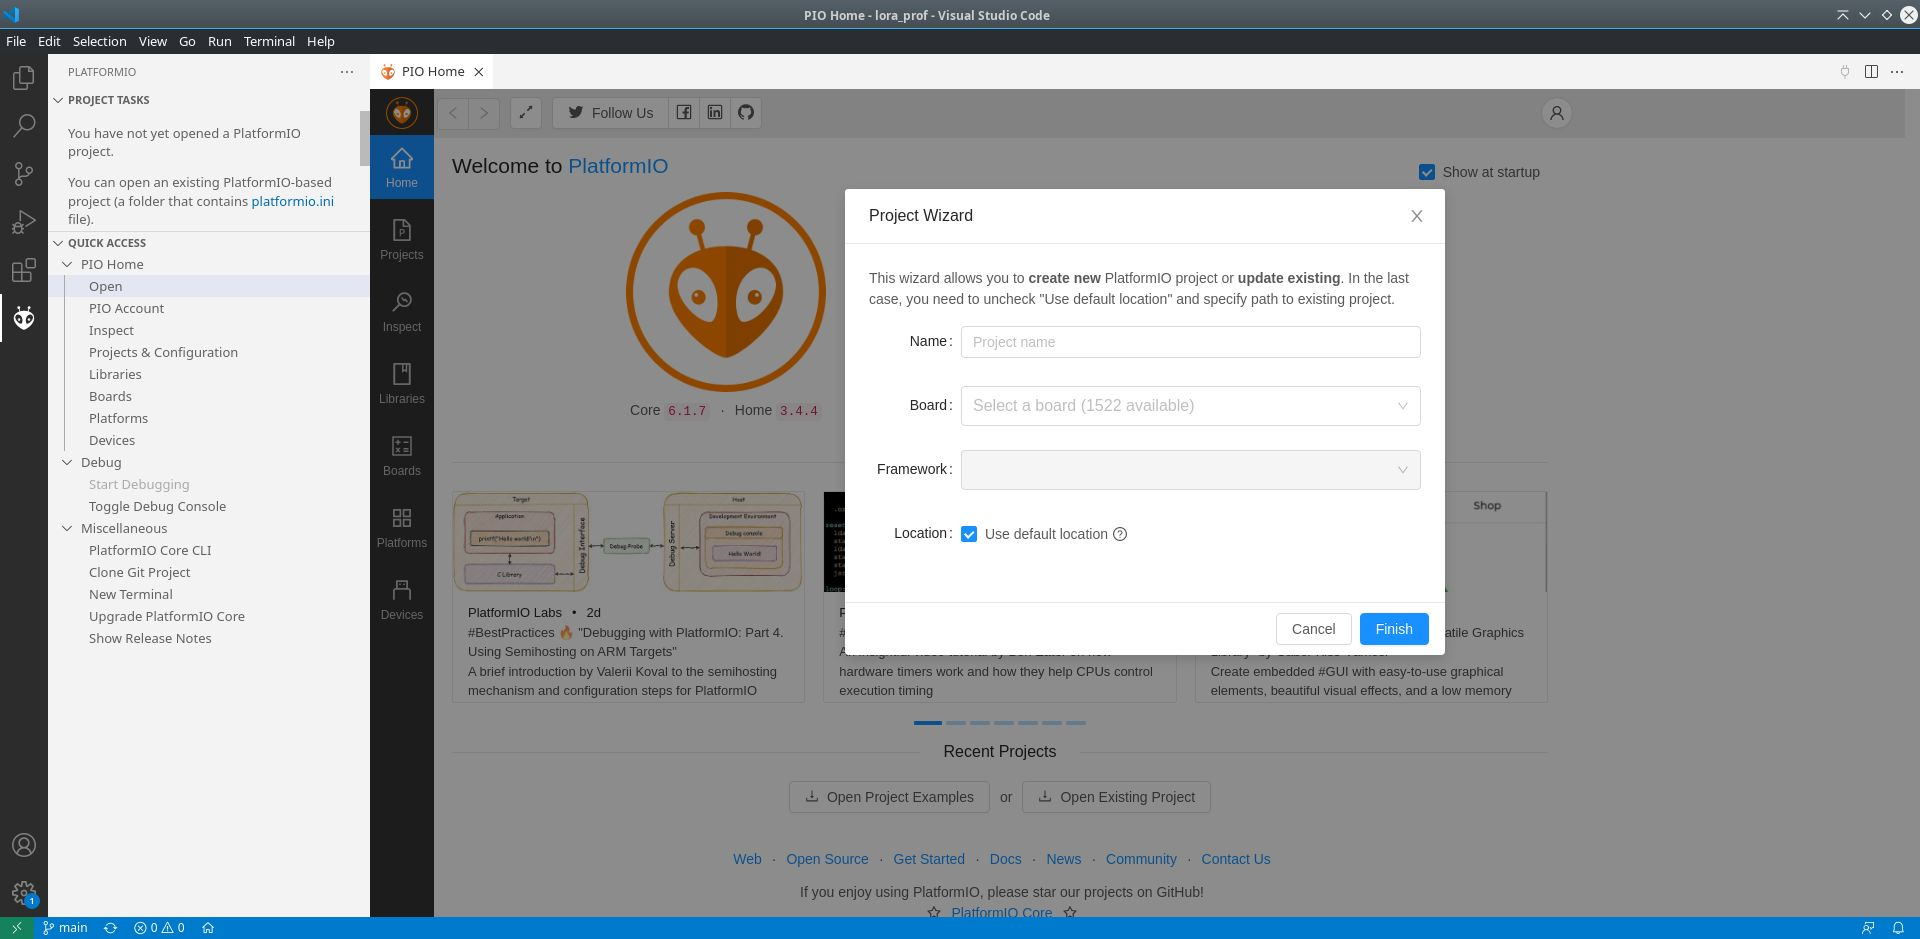
\includegraphics[angle=90, width=10cm]{pic/pio.jpg}
    \end{center}
    \caption{Interfejs narzędzia PlatformIO w edytorze Visual Studio Code}\label{fig:pio}
\end{figure}


\chapter{Istniejące rozwiązania}
W tym rozdziale zostaną przedstawione istniejące rozwiązania, które zostały zaproponowane w~artykułach naukowych i rozwiązaniach komercyjnych.
\section{LoRaWAN}

LoRaWAN (ang. \emph{LoRa Wide Area Network}) to protokół komunikacji stworzony przez LoRa Alliance~\cite{lora:about}.
Protokół ten został stworzony z myślą o~zastosowaniach w sieciach IoT.
Protokół ten jest oparty o~protokół \texttt{LoRa}, i~pozwala na budowę sieci \texttt{LoRa} w~oparciu o~bramy.
Węzły sieci komunikują się z~bramami, a~bramy przekazują dane do serwera.
Serwer jest odpowiedzialny za przetworzenie danych i~przekazanie ich do aplikacji użytkownika.

% \section{The Things Network}

% \section{ChirpStack ?}
% \section{Loriot ?}


\section{Biblioteka \texttt{LoRaMesher}} \label{sec:loramesher}
Badacze w artykule zaproponowali otwartoźródłową implementację autorskiego protokołu \texttt{LoRaMesher}~\cite{bib:loramesher} w postaci darmowej biblioteki.
Biblioteka ta pozwala na budowę sieci opartej o~LoRa bez użycia bram.
Autorzy zaimplementowali protokół w~języku C\texttt{++} z~użyciem systemu FreeRTOS.
Biblioteka została przetestowana na platformie ESP32.

W artykule przedstawiono wyniki testów przeprowadzonych w~rzeczywistych warunkach.
Wiadomości były wysyłane co 120 sekund, a~wiadomości rutingowe co 300 sekund.
Testy zostały przeprowadzone w~trzech różnych scenariuszach:

\begin{itemize}
    \item Sieć złożona z 10 węzłów sieci, oddalone od siebie o~jeden skok. W~takiej sieci wskaźnik dostarczenia pakietów wynosił 90\%.
    \item Sieć złożona z 10 węzłów, ułożonych w~łańcuch (szeregowo). W~tym przypadku wskaźnik dostarczenia pakietów wynosił 96\%.
    \item Sieć złożona z 10 węzłów, w~tym 5~węzłów działało tylko jako przekaźniki. Architektura sieci symulowało użycie biblioteki w~realnym zastosowaniem. W~tym przypadku wskaźnik dostarczenia pakietów wynosił 86\%.
\end{itemize}

Wyniki testów pokazują, że biblioteka działa poprawnie i~może być zastosowana w~prawdziwych zastosowaniach.
Jednak w~artykule nie zostały przedstawione wyniki testów wydajnościowych, które mogłyby pokazać, jak dużo pakietów może być obsłużonych przez bibliotekę.

W odróżnieniu od rozwiązania zaproponowanego w~artykule, w~projekcie zostało zaproponowane rozwiązanie wymagające jednokierunkowej komunikacji z~węzłami sieci.
Dzięki temu można zastosować węzły sieci o~mniejszej wydajności, co pozwala zarówno na zmniejszenie kosztów projektu, jak i~działania węzłów na baterii.

Biblioteka ta została również przygotowana z~myślą o~zastosowaniach, w~których część działania logiki systemu odbywa się na węzłach sieci.
W projekcie zastosowano rozwiązanie, w~którym cała większego systemu jest zaimplementowana w stacji przekaźnikowej i~aplikacji zapisującej do bazy danych.
Dzięki temu można zastosować węzły sieci o~mniejszej wydajności i~zmniejsz poziom skomplikowania systemu.

\section{System monitorowania dużej powierzchni z wykorzystaniem LoRa, oparty o~architekturę typu mesh}

Badacze w podanym artykule~\cite{bib:loramesh-lee} zaproponowali kompletne rozwiązanie umożliwiające monitorowanie dużego obszaru kampusu uniwersyteckiego, w~oparciu tylko o~protokół LoRa.
W odróżnieniu od artykułu opisanego w sekcji~\ref{sec:loramesher} autorzy opisywanego tutaj artykułu zaproponowali rozwiązanie, w~którym to stacja bazowa pobiera dane od poszczególnych węzłów, a~nie węzły samoistnie wysyłają te dane do stacji bazowej.

Główny test został poprzedzony kilkoma mniejszymi testami, które pozwoliły ustalić najlepsze parametry połączenia między węzłami, jak i~ich najlepsze umiejscowienie.

System był testowany przez 8~dni na obszarze 800 na 600 metrów.
Test zawierał jedną stację bazową i~10 węzłów sieci.
Dane były pobierane co 60 sekund.
Wskaźnik dostarczlnośći pakietów uplasował się w~okolicach 88.49\%.

Cechą charakterystyczną tego rozwiązania jest sposób budowania sieci.
Węzeł podczas dołączenia do sieci sam decyduje, przez który z~sąsiadujących węzłów nawiąże komunikacje.
Oczywiście komunikacja może zostać również nawiązana bezpośrednio ze stacją bazową.
Niestety sam proces dołączania nowego urządzenia do sieci i~wyboru węzła-przekaźnika nie jest opisany w tym artykule.
Największą różnicą między tym rozwiązaniem, a~rozwiązaniem zaproponowanym w projekcie jest sposób komunikacji między węzłami.
W projekcie zastosowano rozwiązanie, w~którym węzły nie komunikują się każdy z każdym, a~jedynie z~wybranym węzłem (rodzicem).
Takie rozwiązanie pozwala na zmniejszenie ilości pakietów, które muszą być przetworzone przez węzły sieci, co pozwala na zastosowanie węzłów o~mniejszej wydajności.
Jednak węzły muszą być w stanie komunikować się z~wybranym w~nieznanym procesie rodzicem, co może być problematyczne w~przypadku dużych odległości między węzłami.
Co więcej, w~przypadku zerwania połączenia z~przekaźnikiem, węzeł musi ponownie nawiązać połączenie z siecią, co może prowadzić do straty danych.

Drugą znaczącą różnicą jest sposób komunikacji między węzłami sieci.
W projekcie zastosowano rozwiązanie, w~którym to stacja bazowa odpowiada za pobieranie danych od węzłów sieci.
Jednak w~takim rozwiązaniu stacja bazowa musi być w~stanie obsłużyć wszystkie węzły sieci, co może być problematyczne w~przypadku dużych sieci.
Jeżeli stacja ulegnie awarii, tracone są dane z~wszystkich węzłów sieci.

W przypadku rozwiązania zaproponowanego w~projekcie, stacja bazowa może być zaimplementowana w~taki sposób, aby obsługiwać tylko część węzłów sieci, co pozwala na zastosowanie stacji bazowej o~mniejszej wydajności.
W prosty sposób można również zwiększyć wydajność stacji bazowej, poprzez zastosowanie większej ilości tychże.

\section{Sieć mesh oparta o~LoRa do komunikacji typu \emph{peer-to-peer}}
W artykule~\cite{s21134314} badacze zaproponowali implementację sieci mesh opartej o~protokół LoRa z~wykorzystaniem biblioteki \texttt{RadioHead} i~systemu FreeRTOS na mikrokontrolerach ESP32.
W odróżnieniu od wyżej opisanych artykułów, autorzy zaproponowali rozwiązanie, w~którym to węzły sieci komunikują się ze sobą bezpośrednio, a~nie za pośrednictwem stacji bazowej.
W podanym artykule zostały również przedstawione wyniki testów wydajnościowych, takich jak:
\begin{itemize}
    \item czas potrzebny na przesłanie pakietu między węzłami sieci,
    \item przetwarzanie kilku pakietów między węzłami sieci jednocześnie
    \item skuteczność przesyłu pakietów między węzłami sieci w zależności od odległości między nimi i ustawień transmisji.
\end{itemize}

Wyniki testów pokazują, że biblioteka działa poprawnie i~może być zastosowana w~prawdziwych aplikacjach.
Jednak w~artykule nie zostały przedstawione wyniki testów wydajnościowych, które mogłyby pokazać, jak dużo pakietów może być obsłużonych przez bibliotekę.

Główną różnicą między tym rozwiązaniem a rozwiązaniem zaproponowanym w~naszym projekcie jest sposób komunikacji między węzłami sieci.
W artykule zaproponowano architekturę bez stacji bazowej, więc by dane mogły być przetwarzane poza węzłami sieci, stację bazową należałoby stworzyć we własnym zakresie.
Nie powinno być to trudne, ponieważ mikrokontrolery przesyłają odebrane pakiety przez interfejs UART, więc stacja bazowa mogłaby być zaimplementowana na komputerze PC.


\chapter{Założenia i~implementacja}
W poniższym rozdziale zaprezentowano założenia, potrzeby i~implementację systemu zbierania danych, opartego o~technologię LoRa.

\section{Założenia projektu}
System ma kilka podstawowych założeń:
\begin{itemize}
    \item jeden centralny punkt gromadzenia danych,
    \item zapisywanie danych do bazy danych szeregów czasowych w celu ich dalszego przetwarzania,
    \item zbieranie danych z dużego obszaru,
    \item niezależność od istniejących metod przesyłu danych (WiFi, sieci komórkowe, łączność satelitarna),
    \item niezależność od platformy sprzętowej,
    \item możliwie duża dostarczalność pakietów,
    \item dopuszczalne drobne opóźnienia w dostarczaniu danych.
          % \item węzły sieci tylko wysyłają dane, same nie konsumują przychodzących wiadomości.
\end{itemize}

\section{Części sieci}
W celu uzyskania wyżej wspomnianych założeń, zaproponowano system złożonych z~kilku części:
\begin{itemize}
    \item węzły sieci,
    \item stacje przekaźnikowe,
    \item broker wiadomości,
    \item baza danych.
\end{itemize}

Na rysunku~\ref{rys:system-diagram} przedstawiono schemat systemu.

\begin{figure}[p!]
    \begin{center}
        % 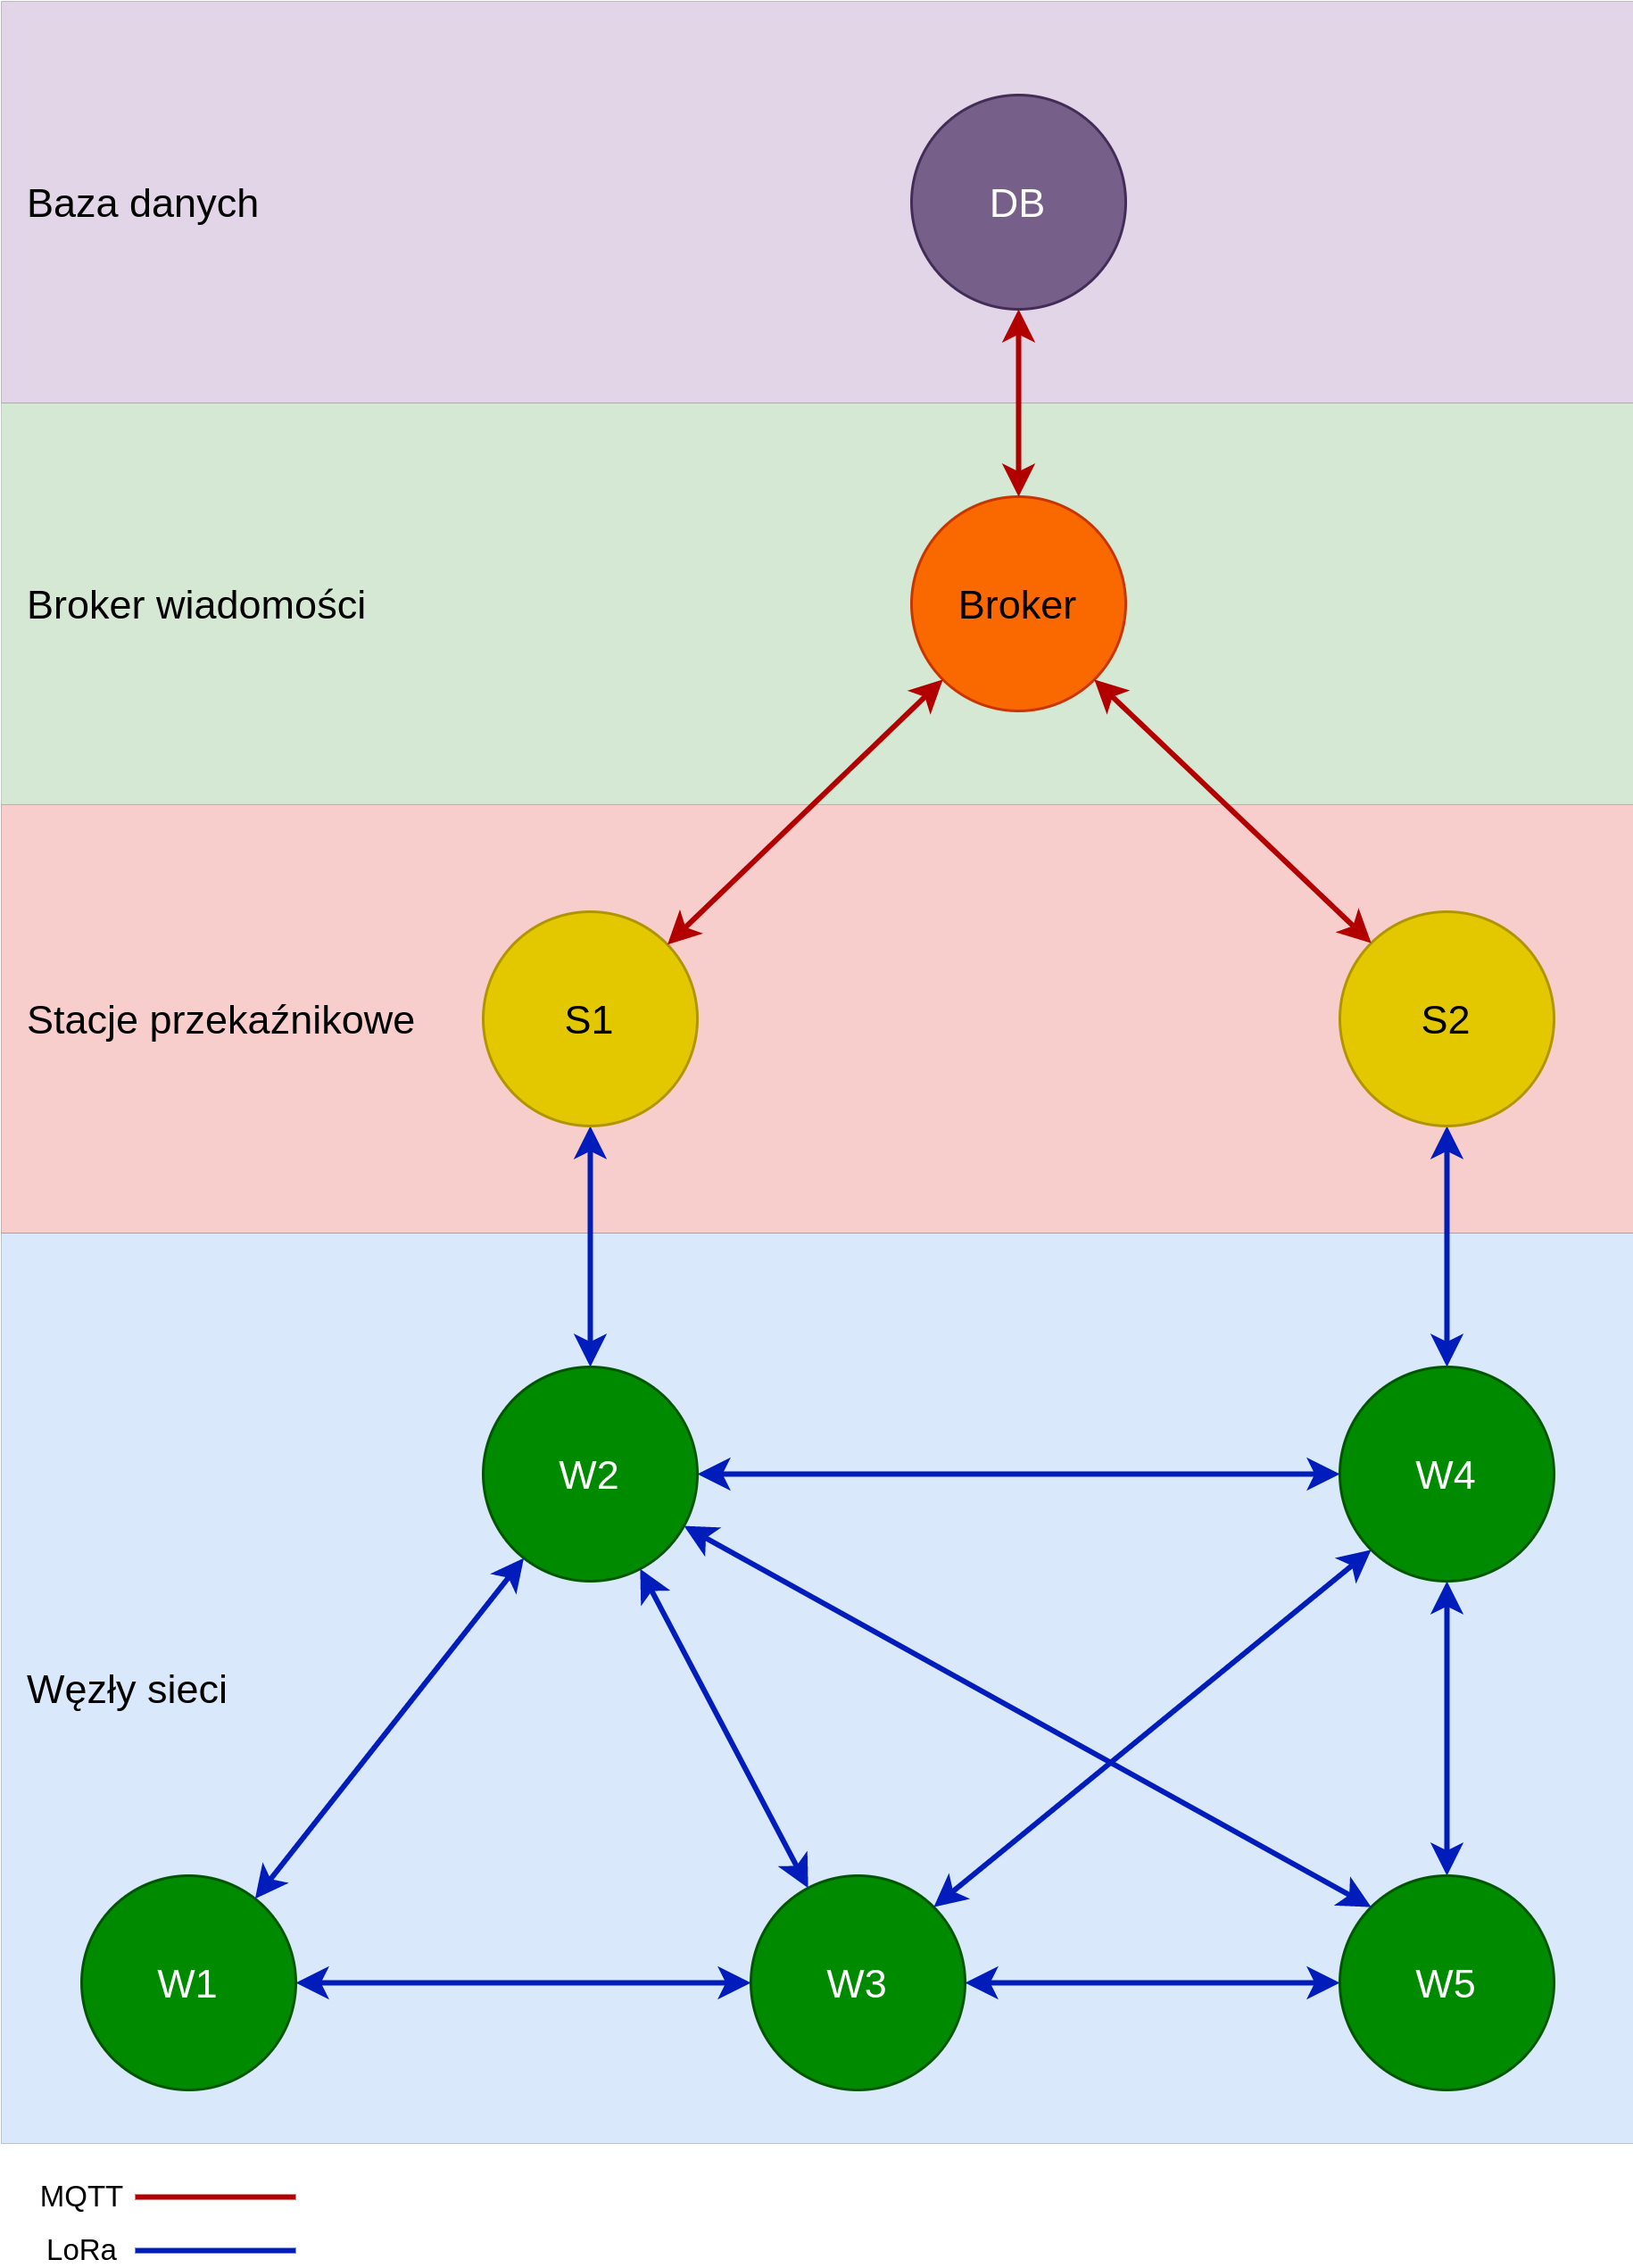
\includegraphics[width=3cm]{pic/diagram-systemu.png}
        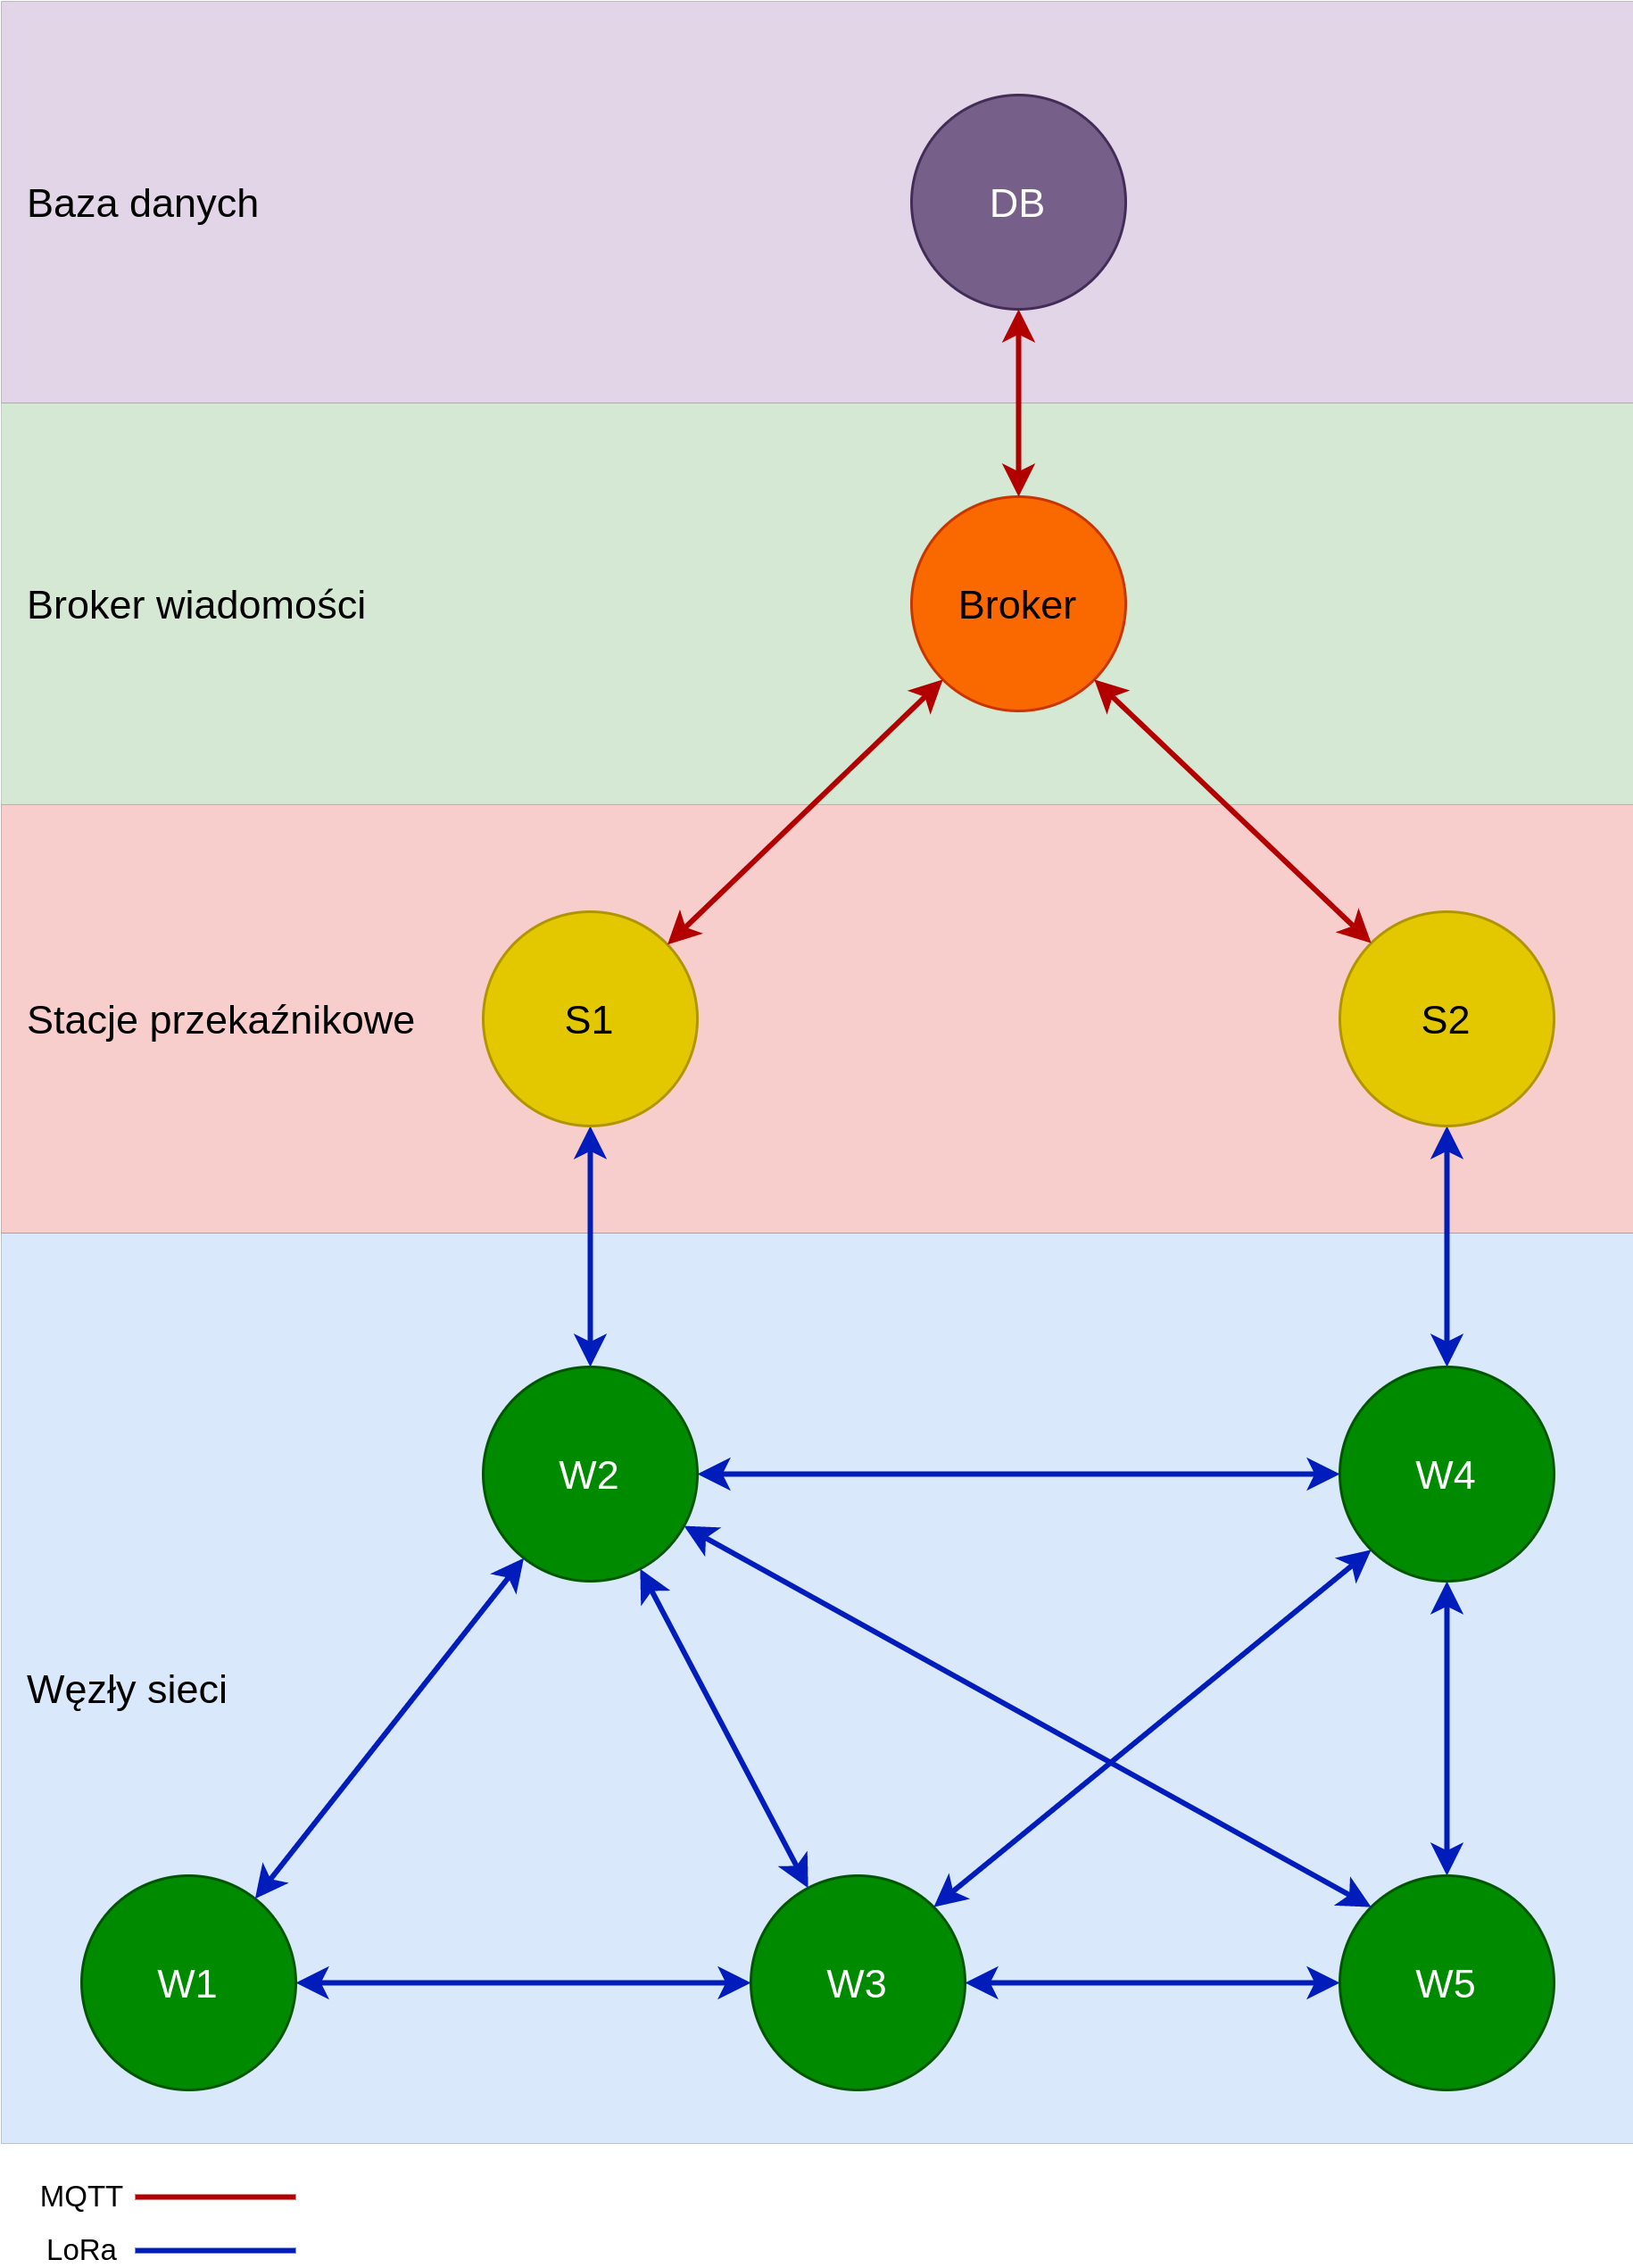
\includegraphics[width=15cm]{pic/diagram-systemu.png}
    \end{center}
    \caption{Diagram prezentujący schemat ideowy systemu}\label{rys:system-diagram}
\end{figure}

\subsubsection{Węzły sieci}
Węzły sieci to urządzenia wyposażone w moduł LoRa i~odpowiednie oprogramowanie pozwalające na pełną obsługę sieci.
Gdy węzeł odbierze wiadomość, sprawdza jej poprawność i~rozsyła ją dalej w celu zapewnienia jak największego zasięgu i~dostarczalności

Urządzenie to może być również wyposażone w~różnego rodzaju czujniki, które dostarczają danych do bazy danych.

\subsubsection{Stacja przekaźnikowa}
Stacja przekaźnikowa to urządzenie wyposażone zarówno w~moduł LoRa, jak i~moduł umożliwiający komunikację z~siecią Internet (np. moduł WiFI lub Ethernet).

Urządzenie to odbiera przychodzące wiadomości LoRa i~przesyła je do brokera wiadomości.

\subsubsection{Broker wiadomości}
Broker wiadomości to program, działający na komputerze mającym dostęp do sieci, umożliwia on wydajną komunikację pomiędzy stacją przekaźnikową a~bazą danych.

\subsubsection{Baza danych}
Baza danych umożliwia zapisywanie sporej ilości danych, uwzględniając również ich czas (baza danych szeregów czasowych).
O~zapis danych z brokera wiadomości do bazy danych dba osobny program, który powinien sprawdzać również poprawność tych wiadomości, jak i~dbać o~to by, nie zapisywać powtórzonych wiadomości.

\section{Wiadomości}
Każda z wiadomości przesyłanych za pomocą tych sieci powinna mieć format jak zaprezentowano na listingu~\ref{lst:packet_format}

Zawiera ona pola:
\begin{itemize}
    \item \texttt{ttl} — (ang. \emph{time to live} — czas życia) wartość określająca maksymalną liczbę skoków pomiędzy węzłami sieci. (domyślnie wynosi 10, może zostać wydłużona w~zależności od wielkości planowanej sieci);
    \item \texttt{m\_id} — UUID~\cite{RFC:uuid} wiadomości, gwarantujący niepowtarzalności tej wiadomości; ułatwia również jej dalsze przetwarzanie;
    \item \texttt{d\_id} — numer identyfikacyjny urządzenia, z~którego pochodzi wiadomość;
    \item \texttt{values} — słownik zawierający dane z~urządzenia, do zapisania w bazie.
\end{itemize}

\begin{lstfloat}[h!]
    % \begin{lstfloat}[b!]
    \lstset{language=JavaScript}
    % \lstset{}
    \begin{lstlisting}[frame=single]
{
    "ttl": 10,
    "d_id": "id_233",
    "m_id": "eaa17a7b-9388-43b6-9310-731c942fc6b9"
    "values": {
        "temp": 21,
        "hum": 50,
        "press": 1000,
        "light": 100,
        "co2": 1000,
        "pm25": 10,
        "pm10": 20
    },
}          
\end{lstlisting}
    \caption{Przykładowa wiadomość przesyłana przez system}\label{lst:packet_format}
\end{lstfloat}

\section{Obsługa protokołu}

\subsubsection{Działanie węzłów}
Wiadomości generowane są przez węzły sieci, zawierając wszystkie niezbędne pola (wymienione wyżej) i~odczyty z czujników zamieszczonych w~węźle.
Następnie zostaje ona rozesłana do wszystkich węzłów w~zasięgu (ang. \emph{broadcasting}).

Węzeł odbierając wiadomość, sprawdza jej poprawność (czy jest odpowiednio sformatowana, czy zawiera wszystkie potrzebne pola), i~jeżeli wiadomość jest poprawna, a~pole \texttt{ttl} jest większe od 0~rozsyła wiadomość dalej.
Sprawdzanie wiadomości odbywa się w~celu wyeliminowania wiadomości niepoprawnych z~sieci.

\subsubsection{Działanie stacji przekaźnikowej}
Stacja przekaźnikowa odbiera wiadomości i~przesyła je do brokera wiadomości.
Nie sprawdza poprawności wiadomości, by zapewnić maksymalną wydajność i~niezawodność.

\subsubsection{Działanie bazy danych i programu zapisującego dane}
Program pobiera kolejne wiadomości od brokera i~przetwarza je w~kolejności:
\begin{enumerate}
    \item sprawdzenie poprawności wiadomości;
    \item \label{itm:powtorki} upewnienie się, czy wiadomość nie została już sprawdzona (na podstawie pola \texttt{m\_id});
    \item zapisanie danych ze słownika \texttt{values} do bazy danych i~przyporządkowanie ich do \texttt{d\_id}, oznaczenie ich znacznikiem czasowym;
    \item zapisanie w pamięci \texttt{m\_id}, potem do wykorzystania w~kroku~\ref{itm:powtorki}.
\end{enumerate}
Baza danych powinna przechowywać dane, takie jak:
\begin{itemize}
    \item \texttt{d\_id} — identyfikator urządzenia,
    \item znacznik czasowy,
    \item wartość pomiaru,
    \item nazwa pomiaru.
\end{itemize}

\section{Implementacja}

\subsection*{Struktura projektu}
Projekt został podzielony na kilka części, które zostały umieszczone w~jednym repozytorium (\url{https://github.com/jasieqb/LoRa-mesh-thesis}).
Repozytorium zostało podzielone na następujące podprojekty:
\begin{itemize}
    \item \texttt{esp32\_node} — implementacja węzłów sieci opartych o~mikrokontroler ESP32,
    \item \texttt{pico\_node} — implementacja węzłów sieci opartych o~mikrokontroler Raspberry Pi Pico,
    \item \texttt{relay} — implementacja stacji przekaźnikowych,
    \item \texttt{influxdb-mqtt-connector} — program zapisujący dane do bazy danych, wraz z plikami konfiguracyjnymi, i definicjami kontenerów Docker, które umożliwiają uruchomienie programu w~kontenerze,
\end{itemize}

\subsubsection{Implementacja węzłów sieci}
W wyniku pracy nad systemem zbierania danych przygotowano implementację węzłów sieci z~wykorzystaniem dwóch platform sprzętowych:

\begin{itemize}
    \item Raspberry Pi Pico,
    \item TTGO LoRa32.
\end{itemize}

\subsubsection{Raspberry Pi Pico}

W wyniku pracy nad systemem zostały przygotowane dwa identyczne urządzenia oparte o~Raspberry Pi Pico.
Urządzenie zostało wyposażone w moduł LoRa SX1262~\cite{PICO:sx1262-doc} (z wykorzystaniem płytki rozwojowej Waveshare SX1262 LoRa Node Module~\cite{PICO:waveshare-doc}) oraz czujnik temperatury i~wilgotności DHT11.
Urządzenie zostało zaprogramowane w~języku MicroPython z~wykorzystaniem biblioteki \texttt{micropySX126X}~\cite{PICO:lora-lib}.
Urządzenie wysyła wiadomości zawierające odczyty z czujnika co 5~minut.
Wysyłanie wiadomości odbywa się w~sposób asynchroniczny, dzięki czemu urządzenie może wykonywać inne operacje w tym czasie. Na listingu~\ref{lst:recive-message} przedstawiono funkcję odpowiedzialną za przetwarzanie przychodzących wiadomości.

\begin{lstfloat}[h!]
    % \begin{lstfloat}[b!]
    \lstset{language=Python}
    % \lstset{}
    \begin{lstlisting}[frame=single]
def handel_msg(msg: bytes):
    logger = Logger()
    msg = msg.decode('utf-8')
    logger.log_info("Message received: {}".format(msg))
    if not check_msg(msg):
        logger.log_error("Message is not valid")
        return
    try:
        msg = json.loads(msg)
    except ValueError:
        logger.log_error("Message is not JSON")
        return

    if msg["d_id"] == GLOBAL_ID:
        logger.log_warning("Message from myself !!!")
        return

    if msg["ttl"] == 0:
        logger.log_warning(f"Message dropped: {msg}, TTL is 0")
        return

    if msg["ttl"] > 0:
        msg["ttl"] -= 1
        msg = json.dumps(msg)
        msg = msg.encode('utf-8')
        time.sleep(random_delay/1000.0)
        sx.send(msg)
        logger.log_info(f"Message forwarded: {msg}")    
\end{lstlisting}
    \caption{Funkcja przetwarzająca przychodzące wiadomości, napisana dla węzłów opartych~o Raspberry Pi Pico}\label{lst:recive-message}
\end{lstfloat}

\subsubsection{TTGO T3 LoRa32}
W wyniku pracy nad systemem zostało przygotowane jedno urządzenie oparte o~TTGO LoRa32.
Urządzenie zostało wyposażone w~moduł LoRa SX1276~\cite{ESP32:sx1276-doc}.
Zostały one zaprogramowane w~języku C++ z użyciem PlatformIO — ekosystemu do programowania urządzeń IoT.~\cite{tool:pio}.
W programie zostały wykorzystane biblioteki:
\begin{itemize}
    \item \texttt{arduino-LoRa} — biblioteka do obsługi modułu LoRa~\cite{ESP32:lora-lib};
    \item \texttt{ArduinoJson} — biblioteka do obsługi formatu JSON~\cite{ESP32:ArduinoJson};
    \item \texttt{Adafruit-SSD1306} — biblioteka do obsługi wyświetlacza OLED~\cite{ESP32:Adafruit-SSD1306};
    \item \texttt{ESPRandom} — biblioteka do obsługi sprzętowego generatora liczb pseudolosowych~\cite{ESP32:ESPRandom}.
\end{itemize}
Urządzenie wysyła wiadomości zawierające odczyty z~czujnika co 5~minut.
Wiadomości zawierają wartości losowe, wygenerowane za pomocą sprzętowego generatora liczb pseudolosowych, zintegrowanego z~mikrokontrolerem ESP32.
Wysyłanie wiadomości odbywa się w~sposób asynchroniczny, dzięki czemu urządzenie może wykonywać inne operacje w~tym czasie. Na listingu~\ref{lst:node_loop} przedstawiono główną pętlę programu.

\begin{lstfloat}[h!]
    % \begin{lstfloat}[b!]
    \lstset{language=C++}
    % \lstset{}
    \begin{lstlisting}[frame=single]
void loop()
{

    unsigned long currentMillis;

    currentMillis = millis();
    if (currentMillis - measurmentMillis >= intervalMeasurment)
    {
        measurmentMillis = currentMillis;
        send_packet();
    }

    if (currentMillis - oledMillis >= intervalOled)
    {
        oledMillis = currentMillis;
        loraDataToOled();
    }

    if (isPacketToResend and (currentMillis - resendMillis >= 
            intervalResend))
    {
        resend_message();
        isPacketToResend = false;
        resendMillis = currentMillis;
    }
    if (isPacketAvailable)
    {
        handle_message();
        isPacketAvailable = false;
    }
}   
\end{lstlisting}
    \caption{Główna pętla programu węzła sieci opartego o~ESP32}\label{lst:node_loop}
\end{lstfloat}

\subsubsection{Implementacja stacji przekaźnikowej}
W wyniku pracy nad systemem zostało przygotowane jedno urządzenie oparte o~płytkę TTGO LoRa32.
Urządzenie zostało wyposażone w~moduł LoRa SX1276~\cite{ESP32:sx1276-doc} oraz moduł WiFi ESP32~\cite{ESP32:datasheet}.
Urządzenie zostało zaprogramowane w~języku C++ z~wykorzystaniem PlatformIO~\cite{tool:pio}.
W programie zostały wykorzystane biblioteki:
\begin{itemize}
    \item \texttt{arduino-LoRa} — biblioteka do obsługi modułu LoRa~\cite{ESP32:lora-lib};
    \item \texttt{Adafruit-SSD1306} — biblioteka do obsługi wyświetlacza OLED~\cite{ESP32:Adafruit-SSD1306};
    \item \texttt{WiFi} — biblioteka do obsługi modułu WiFi ESP32, zawarta w~pakiecie \texttt{arduino-esp32}~\cite{ESP32:Arduino};
    \item \texttt{PubSubClient} — biblioteka do obsługi protokołu MQTT~\cite{ESP32:PubSubClient}.
\end{itemize}

Urządzenie odbiera wiadomości LoRa i~przesyła je do brokera wiadomości za pomocą protokołu MQTT.
Wysyłanie wiadomości odbywa się w~sposób asynchroniczny, dzięki czemu urządzenie może wykonywać inne operacje w~tym czasie.
Urządzenie wyświetla na ekranie OLED informacje o~stanie sieci LoRa oraz otrzymanych wiadomościach.
Urządzenie nie sprawdza poprawności wiadomości, by zapewnić jak największą wydajność i~niezawodność. Na listingu~\ref{lst:callback} przedstawiono funkcję wywoływaną w~reakcji na przerwanie pochodzące~z modułu LoRa.

\begin{lstfloat}[h!]
    % \begin{lstfloat}[b!]
    \lstset{language=C++}
    % \lstset{}
    \begin{lstlisting}[frame=single]
void cbk(int packetSize)
{
    packet = "";
    packSize = String(packetSize, DEC);
    for (int i = 0; i < packetSize; i++)
    {
        packet += (char)LoRa.read();
    }
    rssi = String(LoRa.packetRssi(), DEC);
    loraData();
}
\end{lstlisting}
    \caption{Funkcja wywoływana w reakcji na przerwanie pochodzące~z modułu LoRa, z~stacji przekaźnikowej opartej o~ESP32}\label{lst:callback}
\end{lstfloat}

\subsubsection{Implementacja brokera wiadomości}\label{impl:mosquitto}
Aby zapewnić niezawodność i~wysoką wydajność komunikacji zdecydowano użyć otwartoźródłowego brokera wiadomości Mosquitto~\cite{tool:mosquitto}.
Jest to sprawdzony, wydajny i~niezawodny program, który jest szeroko stosowany w systemach IoT, również w~zastosowaniach profesjonalnych~\cite{tool:mosquitto}.

\subsubsection{Baza danych}\label{impl:db}
W celu zapisywania danych zdecydowano użyć bazy danych InfluxDB 2.0~\cite{tool:influxdb}. Jest to baza danych szeregów czasowych, która jest wydajna i niezawodna~\cite{tool:influxdb}.

\subsubsection{Redis}\label{impl:redis}
W celu przechowywania identyfikatorów wiadomości, które zostały już sprawdzone, zdecydowano użyć bazy danych Redis.
Redis jest szybką, otwartoźródłową, nierelacyjną bazą danych typu \emph{klucz-wartość}, która jest jedną z~najczęściej stosowanych w~systemach informatycznych~\cite{tool:redis}.

\subsubsection{Program zapisujący dane}\label{impl:save}
W celu zapisywania danych zdecydowano użyć programu napisanego w~języku Python.
Program został napisany z~wykorzystaniem bibliotek:
\begin{itemize}
    \item \texttt{paho-mqtt} — biblioteka do obsługi protokołu MQTT~\cite{py:paho-mqtt};
    \item \texttt{influxdb-client} — biblioteka do obsługi bazy danych InfluxDB~\cite{py:influxdb};
    \item \texttt{redis-py} — biblioteka do obsługi bazy danych Redis~\cite{py:redis}.
\end{itemize}

Ostania wymieniona biblioteka została użyta do połączenia się z~bazą danych Redis, w~celu przechowywania identyfikatorów wiadomości, które zostały już sprawdzone.
Dzięki temu program nie zapisuje powtórzonych wiadomości do bazy danych.
Na listingu~\ref{lst:mess-recv} przedstawiono metodę obsługującą przychodzące wiadomości i zapisuje je do bazy danych i Redis.

\begin{lstfloat}[h!]
    % \begin{lstfloat}[b!]
    \lstset{language=Python}
    % \lstset{}
    \begin{lstlisting}[frame=single]
def process_message(self, msg):
    json_msg = parse_json_message(msg)
    if json_msg and  self.valide_message(json_msg) and \
    not self.check_if_processed(json_msg["m_id"]):
        self.save_to_redis(json_msg)
        self.save_to_influxdb(json_msg)
\end{lstlisting}
    \caption{Metoda obsługująca przychodzące wiadomości w programie zapisującym do bazy danach}\label{lst:mess-recv}
\end{lstfloat}


\chapter{Wdrożenie i testy}


\chapter{Perspektywy rozwoju i dalsze badania}

\section{Rozwój projektu}
W~trakcie pracy nad projektem udało się zrealizować wszystkie założenia projektowe.
Wszystkie urządzenia zostały zaprogramowane i~skonfigurowane, a~system zbierania danych został zaimplementowany.
Wszystkie urządzenia zostały przetestowane i~działają poprawnie.
Jednak w~przyszłości można rozwinąć projekt o~kilka funkcjonalności i~usprawnień, które mogą zwiększyć użyteczność systemu.

\subsection{Optymalizacja energetyczna węzłów sieci}
\subsubsection*{Zmniejszenie częstotliwości wysyłania pakietów}
Implementacja węzłów sieci w~obecnej wersji skupia się na stabilności i~poprawności działania.
Jednak w~przyszłości można rozwinąć projekt o~funkcjonalność optymalizacji energetycznej węzłów sieci.
W~obecnej wersji węzły sieci wysyłają pakiety w~stałych odstępach czasu.
Jednak w~przypadku, gdy węzły sieci nie wykryją żadnych zmian w~otoczeniu, nie ma potrzeby wysyłania pakietów.
W~takiej sytuacji można zastosować algorytm, który będzie sprawdzał, czy w~otoczeniu węzła sieci występują jakieś zmiany.
Jeśli nie, to węzeł sieci będzie wysyłał pakiety w~dłuższych odstępach czasu.
Dzięki temu można zaoszczędzić energię węzłów sieci.

\subsubsection{Usypianie węzłów sieci}

Wiele mikrokontrolerów posiada funkcjonalność głębokiego uśpienia.
W~takim trybie mikrokontroler zużywa bardzo mało energii.
Jednak w~takim trybie mikrokontroler nie jest w~stanie wykonywać żadnych operacji.
Należałoby rozpoznać czy tryby uśpienia zaproponowanych przez producentów mikrokontrolerów są wystarczające do zastosowania w~projekcie.
Jeśli tak, to można zastosować tryby uśpienia w~węzłach sieci, które nie będą wysyłały pakietów przez dłuższy czas.

\subsubsection*{Większa bateria}
W celu wydłużenia czasu działania węzłów sieci można również zastosować większe baterie. Wydłużyłoby to nieprzerwany czas pracy na baterii.

\subsubsection*{Zastosowanie innych technologii}
W~celu optymalizacji energetycznej węzłów sieci można również zastosować inne technologie do oprogramowania węzłów sieci.
W~obecnej wersji węzły sieci niektóre węzły sieci zostały zaprogramowane w~języku MicroPython, a~inne w~języku C++.
W~przyszłości można przepisać wszystkie węzły sieci na jeden język programowania.
W~takim przypadku można zastosować język C++, który jest bardziej wydajny od języka MicroPython.
Dzięki temu można zwiększyć wydajność węzłów sieci przy jednoczesnej zwiększonej wydajności energetycznej.
% TODO: dodać bibliografi o wydjaności języków programowania

\subsection{Bezpieczeństwo}

\subsubsection{Autoryzacja węzłów sieci}
W~obecnej wersji systemu węzły sieci nie są autoryzowane.
W~takiej sytuacji każdy węzeł sieci może dołączyć do sieci i~wysyłać pakiety.
Jednak w~przyszłości można rozwinąć projekt o~funkcjonalność autoryzacji węzłów sieci.
Węzły sieci będą musiały autoryzować się przed dołączeniem do sieci.
Dzięki temu można zwiększyć wtedy bezpieczeństwo systemu.

\subsubsection{Szyfrowanie wiadomości}
W~obecnej wersji systemu wiadomości wysyłane przez węzły sieci nie są szyfrowane.
Biorąc pod uwagę specyfikę protokołu LoRa wiadomości są rozgłaszane w formie broadcastu, więc mogą zostać odebrane przez dowolne urządzenie.
W~przyszłości można rozwinąć projekt o~funkcjonalność szyfrowania wiadomości.
W~takiej sytuacji węzły sieci będą szyfrowały wiadomości przed wysłaniem ich do stacji przekaźnikowej.
Następnie stacja przekaźnikowa będzie odszyfrowywała wiadomości przed przekazaniem ich do brokera wiadomości.
Dzięki temu można zwiększyć bezpieczeństwo systemu.

Należałoby rozpoznać, czy szyfrowanie wiadomości nie spowoduje zbyt dużego spadku wydajności systemu.
W~takim przypadku można zastosować szyfrowanie wiadomości tylko w~sytuacji, gdy w~wiadomości znajdują się dane poufne.

Należałoby również sprawdzić, jaka forma szyfrowania jest najbardziej odpowiednia do zastosowania w~projekcie.
W~tym celu można przeprowadzić badania porównujące różne formy i~algorytmy szyfrowania pod względem wydajności i~bezpieczeństwa.

Jeżeli zdecydowano by się na implementacje szyfrowania z~wykorzystaniem klucza, to należałoby rozpoznać, jak klucz będzie przekazywany do węzłów sieci.
W~tym celu można zastosować algorytm wymiany klucza Diffiego-Hellmana.
Dzięki temu klucz szyfrowania będzie przekazywany bezpiecznie.

W celu szyfrowania wiadomości należałoby również rozpoznać, jakie algorytmy szyfrowania są dostępne w~mikrokontrolerach.
W~tym celu można przeprowadzić badania porównujące różne mikrokontrolery pod względem dostępnych algorytmów szyfrowania.

\subsection{Komunikacja dwukierunkowa}
W~obecnej wersji systemu komunikacja między węzłami sieci a~stacją przekaźnikową jest jednokierunkowa.
W~przyszłości można rozwinąć projekt o~funkcjonalność komunikacji dwukierunkowej.
W~takiej sytuacji węzły sieci będą mogły odbierać wiadomości od stacji przekaźnikowej.
Dzięki temu można zwiększyć użyteczność systemu, chociażby poprzez możliwość zdalnego sterowania węzłami sieci.

\subsection{Przygotowanie nowych węzłów sieci}
W~obecnej wersji systemu została przygotowana implementacja węzłów sieci, która jest kompatybilna z~platformami opartymi o Arduino lub MicroPython.
Podczas prac nad następną iteracją projekt można rozwinąć o~funkcjonalność przygotowania nowych węzłów sieci.
W~takiej sytuacji można przygotować implementację węzłów sieci, która będzie kompatybilna z~innymi platformami (takimi jak STM32).
Dzięki temu można zwiększyć uniwersalność systemu.

\section{Dalsze badania}

\subsection{Badania wydajnościowe dużej sieci}
W~trakcie pracy nad projektem zostały przeprowadzone testy wydajnościowe bardzo małej sieci (trzy węzły).
Powinny jednak zostać przeprowadzone badania wydajnościowe dużej sieci.
W~takiej sytuacji można przetestować wydajność systemu w~sytuacji, gdy w~sieci znajduje się dużo węzłów sieci na znacznej powierzchni.
Dzięki temu można sprawdzić, czy system jest w~stanie obsłużyć dużą liczbę węzłów.

\subsection{Badania zużycia energii}
W~trakcie przyszłych prac nad projektem należałoby przeprowadzić badania konsumpcji energii węzłów sieci.
W~takiej sytuacji można sprawdzić, jak długo węzły sieci mogą działać na baterii.
Należałoby również zoptymalizować zużycie energii węzłów sieci.
Dzięki temu można zwiększyć czas działania węzłów sieci na zasilaniu bateryjnym.

\subsection{Badania zasięgu sieci}
W~trakcie przyszłych prac nad projektem należałoby przeprowadzić badania zasięgu sieci.
W~takiej sytuacji można sprawdzić, jak daleko od siebie mogą znajdować się węzły sieci.
Dzięki temu można sprawdzić, jakie są ograniczenia zasięgu sieci.


\chapter*{Podsumowanie}

\addcontentsline{toc}{chapter}{Podsumowanie}


\listof{lstfloat}{Spis listingów} % jeśli są listingi
\addcontentsline{toc}{chapter}{Spis listingów}

% \listoftables{} % jeśli są tabele
% \addcontentsline{toc}{chapter}{Spis tabel}

\listoffigures{} % jeśli są rysunki
\addcontentsline{toc}{chapter}{Spis rysunków}

\printbibliography % wydruk bibliografii
\addcontentsline{toc}{chapter}{Bibliografia} % też ręczne dodanie do spisu treści, jak Wstęp
% \bibliographystyle{plain}
% \begin{thebibliography}{99}
%     \bibitem{bib:a} aaaaaaaa
%     \bibitem{bib:b} bbbbbbbb
%     \bibitem{bib:esp32-all-socs} \href{https://www.espressif.com/en/products/socs}(dostęp: 15.04.2023)
% \end{thebibliography}



\end{document}
